

\section{Einleitung}
\label{sec:intro}

Deep Learning hat bereits in der Vergangenheit bedeutende Fortschritte gemacht, die allesamt wichtige Schritte beim Ausarbeiten einer künstlichen Intelligenz darstellen. Jedoch werden die Lernprozesse innerhalb eines neuronalen Netzwerks oft nur aufbauend von bereits eingespeistem Vorwissen durchgeführt. Somit muss ein neuronales Netz immer gewisse Vorbedingungen kennen, um Problemstellungen zu lösen und kann dabei nicht, wie das menschliche Gehirn, logische Schlüsse ziehen. Betrachtet wird dieses Problem anhand von Erfüllbarkeitsproblemen, welche innerhalb eines tiefer gehenden neuronalen Netzwerks mithilfe eines MAXSAT-Lösers, das Lernen von logischen Zusammenhängen erlauben. Mithilfe dieses Ansatzes, lassen sich somit Problemstellungen lösen, die vorher unmöglich, ohne jegliches Vorwissen an logischen Zusammenhängen von Deep Learning Architekturen, lösbar waren. Die Effektivität dieses Systems wird anhand von drei Beispielen gezeigt, dazu gehört das Lösen von Paritätsfunktionen mit einer Einzelbit-Vorschau und das Lösen eines 9x9 Sudokus, welches zusätzlich noch in handschriftlicher Form vorliegt und dementsprechend mithilfe eines integriertem Zahlen-Erkennungsnetzwerks von einer größeren Architektur gelöst wird. Zusammenfassend zeigen diese Beispiele einen großen Schritt in Richtung logischem Schließen innerhalb Deep Learning Architekturen. 




\section{Ein differenzierbarer Erfüllbarkeitslöser}
\label{sec:sat}
\subsection{SATNet}
\label{sat}
Das MAXSAT-Problem stellt die optimierte Variante des SAT-Problems dar, bei welchem überprüft wird, ob ein logischer Ausdruck lösbar ist. Zum Lösen eines MAXSAT-Problems, wird also die maximale Anzahl an logisch lösbaren Ausdrücken verlangt. Dieses Problem lässt sich darstellen als: 
\[ \sum_{j=1}^m \bigvee_{i=1}^n \boldsymbol{1} \left \{ \tilde{s}_{ij} \tilde{v}_{i} > 0 \right \}\qquad(1),\]
wobei $\emph{n}$ der Variablenanzahl und $\emph{m}$ der Klauselnanzahl einer MAXSAT-Instanz entspricht. Sei $\tilde{v}_{i} \in \{-1, 1\}^n$ der Wahrheitswert der Variable $\emph{i} \in \{1,...,n\}$, und sei $\tilde{s}_{i} \in \{-1, 0, 1\}^m$ mit $\emph{i} \in \{1,...,m\}$, wobei $\tilde{s}_{ij}$ das Vorzeichen von $\tilde{v}_{i}$ in der Klausel $\emph{j} \in \{1,...,m\}$ bestimmt. Es wird in jeder Klausel überprüft, ob der Wahrheitswert \emph{wahr} vorliegt, folglich wird dann eine $\boldsymbol{1}$ aufsummiert. Eine SATNet Schicht nimmt nun als Eingabe diskrete oder probabilistische Zuordnungen von bekannten MAXSAT Variablen und gibt Vermutungen, mithilfe einer \mbox{MAXSAT} SDP Relaxation\cite{https://doi.org/10.48550/arxiv.1706.00476} wieder, was in (Abbildung 1) veranschaulicht wird. \cite[p.~2-3]{https://doi.org/10.48550/arxiv.1905.12149}
\begin{figure}[h]
 \centering
 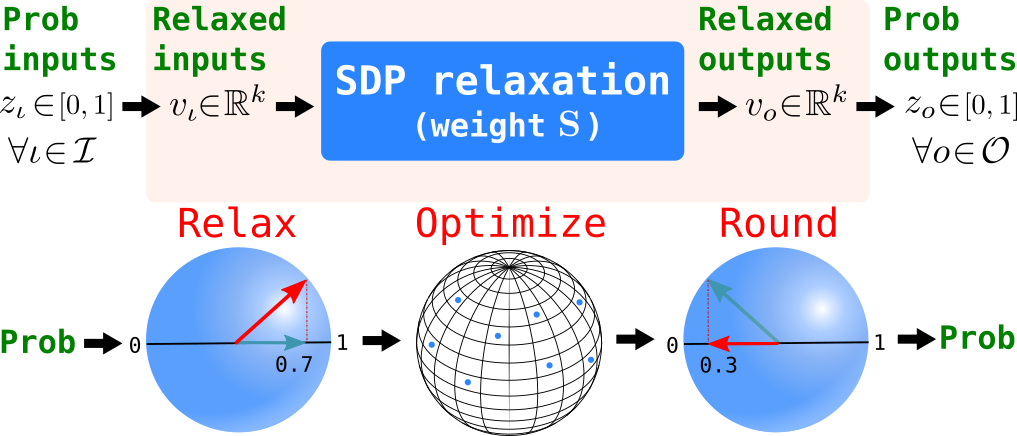
\includegraphics[width=0.65\textwidth]{images/poster_forward.png}
 \caption{SATNet forward pass \cite{githubrepo}}
 \label{fig:forward}
\end{figure}
\subsection{Forward pass}
Sei $\emph{Z}_{\mathcal{I}}$ die Menge aller probabilistischen oder binären Variablen bekannter Zuweisungen mit $\emph{z}_{\emph{i}} \in [0, 1]$ und $\emph{i} \in \mathcal{I}$, mit $\mathcal{I} \subset \{1,...,n\}$. $\emph{Z}_{\mathcal{O}}$ sei die Menge aller probabilistischen oder (optional, zur Testzeit) binären Variablen mit unbekannten Zuweisungen, mit $\emph{z}_{\emph{o}} \in [0, 1]$, und $\emph{o} \in \mathcal{O}$, mit $\mathcal{O} \equiv \{1,...,n\}$~\textbackslash~$\mathcal{I}$. Dabei stellen $\emph{Z}_{\mathcal{O}}$ die aus den Inputs $\emph{Z}_{\mathcal{I}}$ über SDP Relaxation erzeugten Outputs dar.
\label{subsec:forward}
\cite[p.~3]{https://doi.org/10.48550/arxiv.1905.12149}
\subsubsection{Schritt 1: Relaxation der Inputs}
Damit die Inputs $\emph{Z}_{\mathcal{I}}$ als SDP Relaxation anwendbar sind, werden die Inputs $\emph{z}_\emph{i}$ mit $\emph{i} \in \mathcal{I}$ zu zufällig generierten Einheitsvektoren $\emph{v}_{\emph{i}} \in \mathbb{R}^\emph{k}$ relaxiert, wobei mit $\emph{k} = \sqrt{2\emph{n}} + 1$ und mit $\emph{n}$ als Anzahl aller Problemvariablen, die optimale Lösung der MAXSAT Relaxation erzielt wird. Die Gleichung
\[ \emph{v}_{\emph{i}}^\emph{T} \emph{v}_{\top} = -cos(\pi\emph{z}_{i})\qquad(2),\] wird mit
\[ \emph{v}_{\emph{i}} = -cos(\pi\emph{z}_{\emph{i}})\emph{v}_{\top} + sin(\pi\emph{z}_\emph{i})(\emph{I}_{\emph{k}} - \emph{v}_{\top}\emph{v}_{\top}^\emph{T})\emph{v}_{i}^\text{rand}\qquad(3)\] erfüllt.
\cite[p.~4]{https://doi.org/10.48550/arxiv.1905.12149}
\subsubsection{Schritt 2: Erzeugung relaxierter Outputs}
Mithilfe des Koordinatenabstiegs werden Werte für die unbekannten Output Variablen errechnet, dabei besitzt jeder Durchlauf eine Laufzeit von \emph{O}(nmk).
\cite[p.~4]{https://doi.org/10.48550/arxiv.1905.12149}
\subsubsection{Schritt 3: Erzeugung diskreter/probabilistischer Outputs}
Die aus dem Koordinatenabstieg relaxierten Outputs werden mithilfe von zufälligem Runden in die diskreten oder probabilistischen Variablenzuweisungen $\emph{Z}_{\mathcal{O}}$ umgewandelt.
\[ \tilde{v}_{\emph{o}} = \begin{cases}
 & 1 \qquad \quad \text{ wenn } sign($\emph{v}$_\emph{o}^\emph{T}$ \emph{r}$) = sign($\emph{v}$_\emph{$\top$}^\emph{T}$ \emph{r}$) \\ 
 & -1 \qquad \: \text{ andererseits }
\end{cases}, \emph{o} \in \mathcal{O}\qquad(4)\] \emph{r} stellt hierbei eine zufällige Ebene aus der Einheitssphäre dar.
Während der Trainingsphase wird kein zufälliges Runden verwendet, hierbei gilt $\emph{z}_\emph{o} = \emph{P}(\tilde{v}_{\emph{o}})$, mit
\[ \emph{P}(\tilde{v}_{\emph{o}}) = cos^{-1}(-\emph{v}_\emph{o}^\emph{T} \emph{v}_{\top})/\pi \qquad(5).\]
Während der Testphase kann $\emph{z}_{\emph{o}}$ auf die gleiche Art, oder mithilfe von zufälligem Runden, wie in (4), ermittelt werden. \cite[p.~4]{https://doi.org/10.48550/arxiv.1905.12149}
\subsection{Backpropagation}
\label{backward}
Mit den Gradienten $\frac{\partial \emph{l}}{\partial \emph{Z}_{\mathcal{O}}}$, mit \emph{l} als loss des Netzwerks und in Abhängigkeit zu den Outputs $\emph{Z}_{\mathcal{O}}$, lassen sich die Gradienten $\frac{\partial \emph{l}}{\partial \emph{Z}_{\mathcal{I}}}$ in Abhängigkeit der Inputs und $\frac{\partial \emph{l}}{\partial \emph{Z}_{\mathcal{S}}}$ in Abhängigkeit der Gewichte errechnen, um die Anpassungen der Layer Inputs an den entscheidenden Stellen zu tätigen.
\cite[p.~4-5]{https://doi.org/10.48550/arxiv.1905.12149}
\subsubsection{Schritt 1: Von probabilistischen zu realxierten Outputs}
Den Gradienten $\frac{\partial \emph{l}}{\partial \emph{V}_{\mathcal{O}}}$, in Abhängigkeit zu den realxierten Outputs erhält man, in dem man ihn als ($\frac{\partial \emph{l}}{\partial \emph{Z}_{\mathcal{O}}}$) $\cdot$ ($\frac{\partial \emph{l}}{\partial \emph{V}_{\mathcal{O}}}$) umschreibt, wobei sich $\frac{\partial \emph{l}}{\partial \emph{V}_{\mathcal{O}}}$ durch die Ableitung der umgeformten Gleichung aus (5), nämlich als $cos(\pi\emph{z}_{\emph{o}}) = -\emph{v}_{\top}^\emph{T} \emph{v}_{o}$, errechnen lässt.
So erhält man
\[ \frac{\partial \emph{l}}{\partial \emph{V}_{\mathcal{O}}} = \left (\frac{\partial \emph{l}}{\partial \emph{Z}_{\mathcal{O}}}\right) \left(\frac{\partial \emph{z}_{\emph{o}}}{\partial \emph{V}_{\mathcal{O}}}\right) = \left(\frac{\partial \emph{l}}{\partial \emph{Z}_{\mathcal{O}}}\right) \frac{1}{\pi sin(\pi\emph{z}_{\emph{o}})}\qquad (6).\]
\cite[p.~5]{https://doi.org/10.48550/arxiv.1905.12149}
\subsubsection{Schritt 2: Von relaxierten Outputs zu relaxierten Inputs}
Um von den Gradienten $\frac{\partial \emph{l}}{\partial \emph{V}_{\mathcal{O}}}$ zu den Gradienten $\frac{\partial \emph{l}}{\partial \emph{V}_{\mathcal{I}}}$ zu gelangen, wird wie beim forward pass die Prozedur von SDP angewandt.
\cite[p.~5]{https://doi.org/10.48550/arxiv.1905.12149}
\subsubsection{Schritt 3: Von relaxierten zu ursprünglichen Inputs}
Um zu den Gradienten $\frac{\partial\emph{l}}{\partial\emph{Z}_{\mathcal{I}}}$ in Abhängigkeit der ursprünglichen Inputs zu gelangen, werden die Gradienten $\frac{\partial\emph{l}}{\partial\emph{V}_{\mathcal{I}}}$ durch den Schritt 1 aus 3.2.1 geführt, indem Gleichung (3) abgeleitet wird. Man erhält
\[\frac{\partial\emph{l}}{\partial\emph{z}_{\emph{i}}} = \frac{\partial\emph{l}}{\partial\emph{z}_{\emph{i}}^*} + \left ( \frac{\partial \emph{l}}{\partial\emph{v}_{\emph{i}}} \right )^\emph{T} \frac{\partial\emph{v}_{\emph{i}}}{\partial\emph{z}_{\emph{i}}}\qquad(7), \]
wobei 
\[\frac{\partial\emph{v}_{\emph{i}}}{\partial\emph{z}_{\emph{i}}} = \pi(sin(\pi\emph{z}_{\emph{i}})\emph{v}_{\top} + cos(\pi\emph{z}_{i})(\emph{I}_{\emph{k}} - \emph{v}_{\top}\emph{v}_{\top}^\emph{T})\emph{v}_{i}^\text{rand}\qquad(8).\]
\cite[p.~5]{https://doi.org/10.48550/arxiv.1905.12149}



 

\section{Experimente}
\label{sec:results}



\subsection{Lernen von Parität (verkettete XOR)}
\label{subsec:xor}

Dieses Experiment testet das Erlernen SATNets von Parität mit Einzelbit-Vorschau. Dabei soll aus Eingabesequenzen, bestehend aus Bitfolgen die zugehörige Parität ermittelt werden. Das Lernen von Parität war für bisherige konventionelle Deep Learning Architekturen schwer lösbar, aber da das Paritäts-Problem in NP liegt, lässt es sich auf SAT reduzieren. Das Modell ist dabei so aufgebaut, dass es bei einer Länge von $L$ eine Anzahl von $L$ - 1 SATNet Schichten, mit gebundenen Gewichten enthält. Dabei nimmt die erste Schicht die ersten beiden Binärwerte der Bitfolge als Input. Die Schicht $d$ nimmt dabei den Binärwert $d$ und zusätzlich den gerundeten Output der Schicht $d$ - 1 als Input. Sobald jede einzelne Schicht das Berechnen von XOR-Funktionen erlernt hat, wir das gesamte Modell die korrekte Parität ausgeben. Um diese Ausgaben zu erlangen muss das System erst eine lange Abfolge von SAT-Problemen bearbeiten. Für die vorgegebenen Längen von $L$ = 20 und $L$ = 40 wird ein zufällig generierter Datensatz von zehntausend Beispielen erzeugt, 9000 davon werden dem System als Trainingseinheit gegeben und 1000 schließlich als Testeinheit. Verglichen mit einem LSTM-Sequenzklassifizierer erzielt das SATNet hierbei deutlich bessere Ergebnisse (Bild 2). LSTM ist nicht dazu in der Lage eine angemessen Darstellung der Parität zu lernen und hat auch im Laufe von 100 Trainingsepochen keine signifikante Verbesserung erzielt. Über beide Input-Längen erzielt LSTM dabei nur eine Testerrorrate von bestenfalls 0,476 (Ein zufälliges Raten hätte eine Rate von 0,5). \cite[p.~6]{https://doi.org/10.48550/arxiv.1905.12149}

\begin{figure}[h]
 \centering
 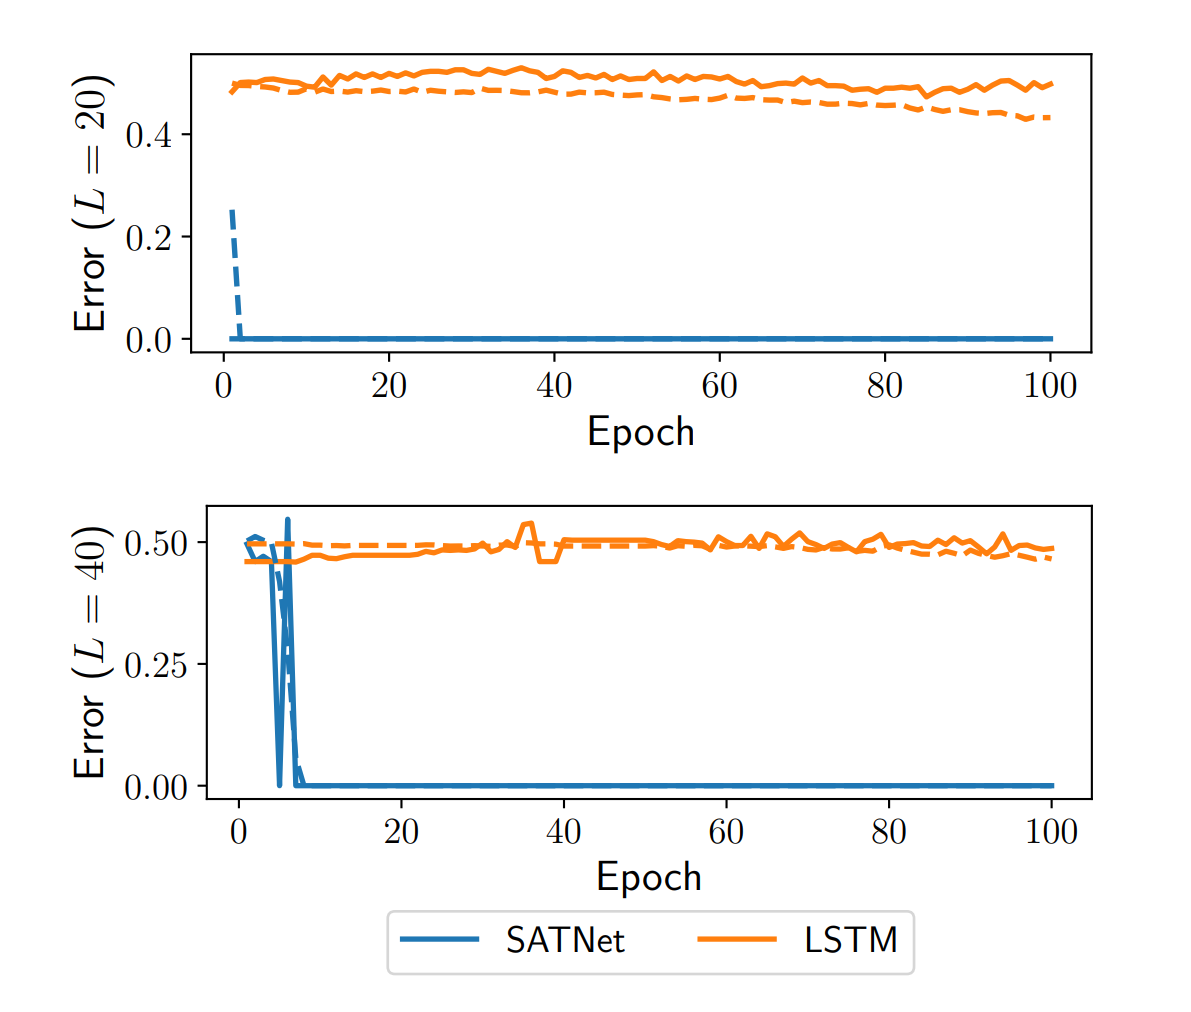
\includegraphics[width=0.65\textwidth]{images/SATNet_LSTM_graph.png}
 \caption{Fehlerrate des Paritätsexperiments \cite[p.~6]{https://doi.org/10.48550/arxiv.1905.12149}}
 \label{fig:parity}
\end{figure}




\subsection{Sudoku (original und permutiert)}
\label{subsec:sud}

Sobald die Regeln von Sudoku bekannt sind, lässt sich das Problem rechnerisch leicht bewältigen. Die eigentliche Herausforderung stellt dabei das Erlernen der Regeln dar, was ebenfalls für konventionelle neuronale Netzwerke Probleme dargestellt hat. Normalerweise wurden Sudoku Problemstellungen über Baumsuchen gelöst, diese lassen sich jedoch schlecht in neuronalen Netzen Ausführen, sind aber leicht als SAT oder MAXSAT Probleme darzsutellen. Dem SATNet wird hierbei als Input eine logische Bitdarstellung geliefert, welche zudem die zu lernenden Bits, also die unbekannten Felder im Spielfeld, darstellt. Der Output besteht folglich wieder aus einer Bitdarstellung mit zufällig Gewählten Eingaben für die unbekannten Bits. Erneut wurden für dieses Experiment 9000 Trainingsbeispiele und 1000 Testbeispiele erzeugt, welche bei SATNet nach 100 Trainingsepochen zu einer Genauigkeit von 98,3\% führten. Verglichen mit dem faltenden neuronalen Netzwerk "ConvNet", löst dieses die Trainingseinheiten mit einer Genauigkeit von 72,6\%, die eigentlichen Testeinheiten jedoch nur mit 0,04\%. 
Um sich nun zu vergewissern, dass SATNet nicht einfach nur gewisse Strukturen in der Eingabe erkennt, sondern tatsächlich die Sudokuregeln lernt, wurde das Experiment mit einer permutierten Version, bei der die Eingaben entsprechend angepasst wurden, erneut ausgeführt. Durch die Permutation liegen keine erkennbaren Strukturen innerhalb der Eingabe vor, die Spielregeln von Sudoku und die logischen Zusammenhänge der Eingabe bleiben jedoch bestehen. SATNet hat unter diesen Bedingungen erneut eine Genauigkeit von 98,3\% erzielt und zeigt somit, dass diese Architektur dazu in der Lage ist die Spielregeln zu erlernen und anzuwenden. ConvNet hingegen erzielte bei dem permutierten Test eine null prozentige Genauigkeit. 
\cite[p.~6-7]{https://doi.org/10.48550/arxiv.1905.12149}

\subsection{Visuelles Sudoku}
\label{subsec:visSud}
Um nun die Integration von SATNet in größeren Architekturen zu zeigen, werden in einem Experiment die SATNet-Schichten mit denen eines faltenden neuronalen Netzwerks kombiniert, welches für die Erkennung eines visuell vorliegenden Sudoku-Spielfeld nötig ist. Der Output dieser Schichten wird SATNet als logischer Input geliefert, wie in 4.2. Hierzu findet wieder ein Vergleich zu einer ConvNet Architektur statt, wobei der Ablauf der Zahlenerkennung gleich verläuft. Unter denselben Trainingsbdingungen kann eine maximale Genauigkeit von 74,7\% erreicht werden, was der einhergehenden visuellen Erkennung verschuldet ist. Nach 100 Epochen erzielt die SATNet Architektur eine Genauigkeit von 63,2\%, was 85\% des theoretischen Optimums entsprechen. Das ConvNet besitzt nach 100 Epochen keine nennenswerte Genauigkeit und kann keine sinnvollen Lösungen liefern. So ist es der gesamten Architetkur, dank dem SATNet auch möglich die Sudokuregeln von einer handschriftlich vorliegenden Repräsentation zu lernen, was zuvor nicht möglich war. \cite[p.~7-8]{https://doi.org/10.48550/arxiv.1905.12149}

\section{Folgerung}
\label{sec:conclusion}
In dieser Arbeit wird die Funktionsweise der SATNet Schicht präsentiert, die dazu in der Lage ist Erfüllbarkeitsprobleme zu lösen, wie in den Experimenten der Parität und dem Erlernen der Sudoku Spielregeln veranschaulicht wird. Zudem wurde mit dem Experiment des visuellen Sudokus gezeigt, dass sich diese Schicht auch in größere Deep Learning Architekturen integrieren lässt, was diesen die Möglichkeit gibt, logische Zusammenhänge zu erlernen, ohne dabei auf hinzugegebene Informationen zurückzugreifen. Das tatsächliche Erlernen von logischen Zusammenhängen konnte in den bisherigen Deep Learning Architekturen nicht überzeugend umgesetzt werden. SATNet zeigt jedoch hierbei große Fortschritte im Erlernen dieser Zusammenhänge und stellt dabei einen wichtigen Teil des Deep Reasoning dar.





